\footnotesize
\begin{tikzpicture}[>=latex]
\begin{axis}[
width=7cm,
height=7cm,
xtick=\empty,
ytick=\empty,
axis x line=center,
axis y line=center,
xlabel={$\dfrac{M^*}{\phi{}M_s}$},
ylabel={$\dfrac{V^*}{\phi{}V_v}$},
xlabel style={right},
ylabel style={left},
xmin=-.2,xmax=1.2,ymin=-.1,ymax=1.2]
\draw[ultra thick](axis cs:0,1)node[left]{\num{1}}--(axis cs:.75,1)--(axis cs:1,.6)--(axis cs:1,0)node[below]{\num{1}};
\draw[dashed](axis cs:0,.6)node[left]{\num{0.6}}--(axis cs:1,.6);
\draw[dashed](axis cs:.75,0)node[below]{\num{0.75}}--(axis cs:.75,1);
\end{axis}
\end{tikzpicture}